\documentclass{article}
\usepackage[utf8]{inputenc}
\usepackage{graphicx}
\graphicspath{ {./images/} }
\usepackage{hyperref}
 \usepackage{amsmath} 
\usepackage[legalpaper, portrait, margin=0.5in]{geometry}

\title{Bravo Torque Control}
\author{Carlos Suarez Zapico}
\date{August 2025}

\begin{document}

\maketitle

\section{Introduction}

\begin{equation}
    \begin{align*}       
    
        \mathbf{F}_{\text{task}} = \mathbf{K}_x (\mathbf{x}_{\text{des}} - \mathbf{x}) + \mathbf{D}_x (\dot{\mathbf{x}}_{\text{des}} - \dot{\mathbf{x}}) \\
    
        \boldsymbol{\tau}_{\text{task}} = \mathbf{J}^\top \mathbf{F}_{\text{task}} \\


        \label{eq:impedance_dof}    
    \end{align*}
\end{equation}

\begin{equation}
        \mathbf{K}_x = \begin{bmatrix}
        k_x & 0 & 0 \\
        0 & 0 & 0 \\
        0 & 0 & k_z
        \end{bmatrix}
    \label{eq:SelectTaskDimensions}
\end{equation}

\begin{equation}
    \ddot{\mathbf{x}}_{\text{des}} = \mathbf{M}^{-1} \left( \mathbf{F}_{\text{ext}} - \mathbf{D}_x \dot{\mathbf{x}} - \mathbf{K}_x (\mathbf{x} - \mathbf{x}_{\text{eq}}) \right)
\end{equation}

\section{Stiction}

\subsection{Approach 1: Friction feedforward (with Stribeck)}

Identify static friction torque $\tau_s$ per joint. Apply it in the command before feedback kicks in.  For example:
\begin{equation}
    \tau_{\text{cmd}} = \tau_{\text{ctrl}} + F_s \cdot \text{sgn}_\epsilon(\dot{q})
\end{equation}


where $\text{sgn}_\epsilon$ is a smooth sign function to avoid chatter. This lets you lower feedback gains but still overcome the threshold.

\subsection{Approach 2}
\subsubsection{Separate loops + keep the outer one soft} 
\begin{itemize}
    \item Inner loop: fast current (torque) control. Aim for high bandwidth and good disturbance rejection here.
    \item Outer loop: low-gain impedance/admittance layer that commands torque, not position. Use a virtual spring-damper: $\tau_c = K_p(q_{ref} - q) + K_d(\dot{q_{ref} - \dot{q}})$. Keep $K_p$,$K_d$ modest for compliance, then add smart feedforward so you don’t need big gains.
\end{itemize}


\subsubsection{Put friction in the feedforward path (not the feedback)}
Model + compensate for the stuff that’s forcing you to raise gains.
Simple friction model (good start):
\begin{equation}
    \tau_f = F_c \text{sgn}(\dot{q}) + B\dot{q} + (F_s - F_c) e^{-(\dot{q}/v_s)^2} \text{sgn}(\dot{q})
\end{equation}

Then command:
\begin{equation}
    \tau_{cmd} = \tau_c + \tau_f +\tau_g
\end{equation}

where $\tau_g$ is gravity compensation (from your model or ID’d offline).

If you don’t want to fit Stribeck yet, start with Coulomb + viscous (two parameters per joint). Identify by sweeping at slow velocities in both directions and solving for 
$F_c$ and $B$. 
Implementation tips: Estimate $\dot{q}$ with a well-tuned low-pass differentiator/observer (e.g., 2nd-order Butterworth with cutoff comfortably above motion bandwidth, below current loop bandwidth). Blend friction near zero speed to avoid sign chatter:
\begin{equation}
    \text{sgn}_\epsilon(\dot{q}) = \frac{\dot{q}}{\sqrt{\dot{q}^2 +\epsilon^2}}
\end{equation}

\subsubsection{Use a tiny “dither” to break stiction (optional but effective)}
Inject a small sinusoidal current at a few Hz (or just above your mechanical resonance) when $|\dot{q}>0|$ and $∣q\*−q∣>0$. Amplitude: just enough to exceed stiction (a few percentage of rated torque). Gate it off once motion starts. This reduces stick-slip without raising gains.

\begin{itemize}
    \item Add a small high-frequency torque (a few percentage of rated torque) around zero velocity.
    \item Frequency: above your motion bandwidth but below mechanical resonances (often 20–80 Hz for small arms).
    \item Effect: Keeps micro-motion at contact points so surfaces never “fully stick.”
\end{itemize}

\begin{figure*}[h!]
\begin{center}
     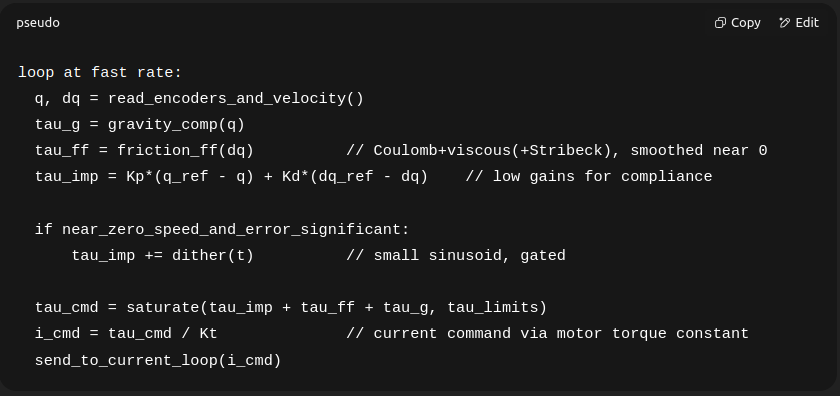
\includegraphics[width=\linewidth]{images/Selection_083.png}
     \caption{PseudoCode}
     \label{fig:PseudoCode}
\end{center}
\end{figure*}

\vspace{5cm}
\section{Stribeck Effect}
The Stribeck effect is a phenomenon in friction where the friction force decreases as speed increases from zero. It is basically the transition from “sticky” to “slippery.”

\subsection{What’s going on physically?}

At zero velocity, static friction (stiction) dominates — it takes a certain torque/force just to break loose. As soon as motion starts, the contact surfaces shift from “micro-welded” to “sliding with a thin lubricant film” or micro-rolling, so the required force drops — this is the Stribeck region. After that drop, viscous friction (proportional to speed) takes over, so total friction rises again at higher speeds.

\subsection{Mathematical Model}
\begin{equation}
    F_f(\dot{q}) = \left[F_c + (F_s - F_c) e^{-(\dot{q}/v_s)^2}\right] \text{sgn}(\dot{q}) + B\dot{q}
\end{equation}
where:
\begin{itemize}
    \item $F_s$ static friction
    \item $F_c$ Coulomb (constant sliding) friction
    \item $v_s$ Stribeck velocity (where drop happens)
    \item $B$ viscous coefficient
\end{itemize} 

\subsection{Why it matters for robot control}
\begin{itemize}
    \item If you ignore it, your low-speed torque commands will overshoot → jerky starts/stops. 
    \item When trying to control low contact forces or track slow motions (especially in current control), Stribeck friction is the main reason you need higher gains to break stiction — and higher gains kill compliance. 
    \item Modeling + feedforward compensating for it lets you run much lower position/impedance gains while still moving smoothly.
\end{itemize}

Stiction (static friction) is particularly nasty because:
\begin{itemize}
    \item In \textbf{free motion}: you need a sudden torque jump to break loose → jerk, overshoot, buzzing.
    \item In \textbf{force control}: near zero velocity, the joint “sticks” until the commanded force exceeds static friction, then it “slips” and overshoots the target force — classic stick–slip instability.
\end{itemize}

\begin{itemize}
    \item \textbf{Nonlinearity}: Unlike viscous friction (smooth, proportional to velocity), static friction is a discontinuous threshold. Your controller can’t just scale output linearly — it’s like pushing a stubborn door: nothing happens until suddenly everything moves.
    \item \textbf{Deadzone Effect}: If your desired torque is below  (the static friction torque), nothing moves. This destroys your ability to apply gentle forces or track small motions.
    \item \textbf{Force ripple}: In contact, the “break–slip–stick” cycle makes your force measurement oscillate instead of staying constant.
\end{itemize}

\begin{figure*}[h!]
\begin{center}
     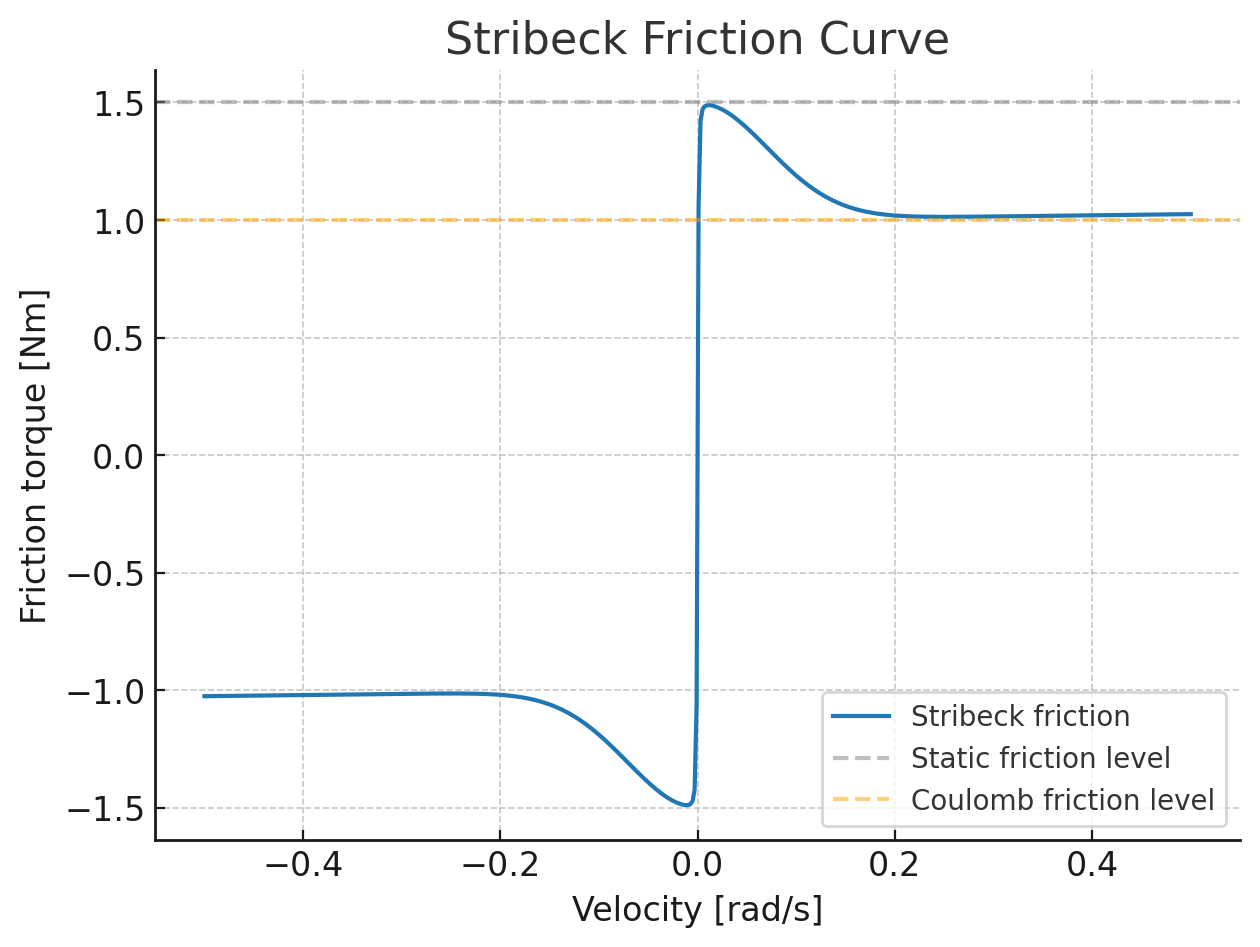
\includegraphics[width=\linewidth]{images/stribeck.png}
     \caption{Stribeck}
     \label{fig:Stribeck}
\end{center}
\end{figure*}
Here’s the Stribeck curve — you can see the peak at zero speed (static friction), then the drop toward the sliding level as speed increases, and finally the viscous slope at higher velocities. This “sticky → slippery” transition is exactly what causes jerky starts and stick–slip.

\section{Stiction}



\end{document}
